% Dokumentklassen s�ttes til memoir.
% Manual: http://ctan.org/tex-archive/macros/latex/contrib/memoir/memman.pdf
\documentclass[a4paper,oneside,article]{memoir}

\usepackage{pgf}
\usepackage{tikz}
\usepackage{pgfplots}
\usetikzlibrary{arrows,automata}
\usepackage{verbatim}
 
% Danske udtryk (fx figur og tabel) samt dansk orddeling og fonte med
% danske tegn. Hvis LaTeX brokker sig over �, � og � skal du udskifte
% "utf8" med "latin1" eller "applemac". 
\usepackage{inputenc}
\usepackage[danish]{babel}
\usepackage[T1]{fontenc}
 
% Matematisk udtryk, fede symboler, theoremer og fancy ting (fx k�debr�ker)
\usepackage{amsmath,amssymb}
\usepackage{bm}
\usepackage{amsthm}
%\usepackage{mathtools}
 
% Kodelisting. Husk at l�se manualen hvis du vil lave fancy ting.
% Manual: http://mirror.ctan.org/macros/latex/contrib/listings/listings.pdf
\usepackage{listings}
 
% Fancy ting med enheder og datatabeller. L�s manualen til pakken
% Manual: http://www.ctan.org/tex-archive/macros/latex/contrib/siunitx/siunitx.pdf
%\usepackage{siunitx}
 
% Inds�ttelse af grafik.
\usepackage{graphicx}
\usepackage{float}
 
% Reaktionsskemaer. L�s manualen for at se eksempler.
% Manual: http://www.ctan.org/tex-archive/macros/latex/contrib/mhchem/mhchem.pdf
%\usepackage[version=3]{mhchem}
%\usepackage[noend]{algpseudocode}
%\usepackage{algorithm}

\usepackage{xcolor,colortbl}

\usepackage{listings}

\definecolor{javared}{rgb}{0.6,0,0} % for strings
\definecolor{javagreen}{rgb}{0.25,0.5,0.35} % comments
\definecolor{javapurple}{rgb}{0.5,0,0.35} % keywords
\definecolor{javadocblue}{rgb}{0.25,0.35,0.75} % javadoc

\lstset{language=Java,
basicstyle=\small, %\ttfamily,
keywordstyle=\color{javapurple}\bfseries,
stringstyle=\color{javared},
commentstyle=\color{javagreen},
morecomment=[s][\color{javadocblue}]{/**}{*/},
numbers=left,
numberstyle=\tiny\color{black},
stepnumber=1,
numbersep=10pt,
tabsize=4,
showspaces=false,
showstringspaces=false}

\begin{document}
    \title{Naming - Disposition}
    \author{Lukas Peter J�rgensen, 201206057, DA4
            }
    \maketitle
    
    \chapter{Terminology}
    \begin{itemize}
    \item[Entity] A machine, a process, a file etc.
    \item[Access point] An entity at which other entities can be located. \\E.g. a process can be located at a given machine.
    \item[Name] A string of bits or characters that is used to refer to an entity
    \item[Address] A name that refers to an access point of an entity
    \item[Identifiers] A name which uniquely identifies an entity
    \item[Human-friendly names] A character string name that is understandable by a human.
    \item[Flat naming] Name gives no hints on location (E.g. a random string like 00:11:22:33)
    \item[Structured naming] Name describes how to locate object (E.g. a URL)
    \item[Attribute-based naming] E.g. /C=DK/O=AU/OU=Comp.Sc.
    \end{itemize}
    
    \chapter{Flat names}
    \section{Address Resolution Protocol (ARP)}
    \textbf{Name:} IP Address, the "logical name" at this level.\\
    \textbf{Address:} MAC Addres, the accesss point on the ethernet network\\
    \textbf{Method:}
    \begin{itemize}
    \item Machines know their name and address.
    \item To locate the address with name $N$, broadcast a packet $P$ with $N$.
    \item Receivers check whether they have name $N$ and if so, report back with their address.
    \end{itemize}
    
    \section{Mobility}
    \begin{itemize}
    \item Name constant.
    \item Access point changes.
    \end{itemize}
    
    \subsection*{Solutions}
    \textbf{Using an ARP-like protocol}, the entity could multicast new location to group when it has moved, or the node can broadcast for new location of entity when needed.\\
    \\
    \textbf{Forwarding pointers}, leave a breadcrumb everytime the entity moves from A to B, so clients can find the entity at B by following the breadcrumb at A that point to B.\\
    \textbf{Pros:} Simplicity\\
    \textbf{Cons:} If the entity is highly mobile, the trail can become very long, the trail has to be maintained at every crumb. It's very vulnerable as well, if one crumb is missing, the whole chain is broken.\\
    \\
    \textbf{Home-based approach}, have a static home agent, that redirects all to an ip-address that the mobile-host can update when it receives a new ip address.\\
    \textbf{Cons:} If the mobile-host is permanently moved far away from the home-host, then requests will take a longer time than if the home-host had moved with it.
    
    \chapter{Distributed Hash Table}
    $succ(key)=$ smallest identifier larger than $key$.\\
    E.g. if identifiers $= \{1,4,7,12,15\}$ then $succ(9)=12$ and $succ(12)=12$\\
    \\
    \textbf{Lookup:} Given $key$, find $succ(key)$ and the address of the peer with identifier $succ(key)$. Na�ve solution takes time $O(N)$
    \section*{Finger tables}
    \begin{figure}[H]
    \centering
    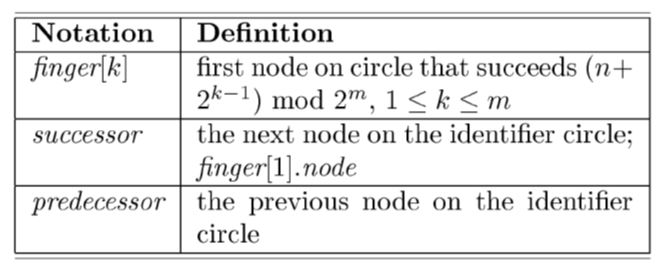
\includegraphics[width=\textwidth]{Media/FingerDef.jpg}
    \end{figure}
\end{document}